\documentclass[10pt]{article}

\usepackage{polski}
\usepackage{graphicx}
\usepackage{hyperref}
\graphicspath{{images/}}
\usepackage{mathtools}

\usepackage{geometry}
\newgeometry{tmargin=4cm, bmargin=4cm, lmargin=3.2cm, rmargin=3.2cm} 

\usepackage{fancyhdr}
\pagestyle{fancy}

 

\begin{document}


\begin{titlepage}
\begin{center}
  
  \LARGE \textsc{Politechnika Wrocławska}\\
  \vspace*{0.2cm}
  \Large \textsc{Wydział Informatyki i Telekomunikacji}\\  
  \vspace*{0.4cm}
  \centering
\includegraphics[width=0.2\textwidth]{WITlogo.png}\\
  \vspace*{0.2cm}
  \vspace*{2cm}
        
  \centerline{\rule{\textwidth}{1.2pt}}
  \vspace{0.4cm}
  \Huge\textbf{Regresja danych dotyczących zarybiania zbiorników wodnych}
  \centerline{\rule{\textwidth}{1.2pt}}
  \vspace{1cm}
  \LARGE Sprawozdanie z laboratorium MSiD\\
  \vspace{3.5cm}
  \textsc{Autor}\\
  \vspace{0.2cm}
  \textbf{Ryszard Polkowski}\\
  \vspace{0.1cm}
  \Large nr albumu: \textbf{260376}\\
  \vspace{0.1cm}
  kierunek: \textbf{Informatyka Stosowana}
            
            
        
        
  \vspace*{\fill}
  \Large \textit{7 czerwca 2022}
            
 \end{center}


\end{titlepage}

\begin{abstract}

Praca przedstawia program do wyliczania regresji liczby ryb wykorzystanych do zarybiania zbiorników wodnych. Działa on dzięki danym ze strony \url{https://data.ny.gov}. Dane zostały oczyszczone ze zbędnych wierszy nie posiadających kompletnych informacji oraz z kolumn posiadających dane zależne od innych kolumn. Następnie zostały z nich wylosowane wiersze do predykcji liczby ryb na podstawie przybliżonej daty, zbiornika wodnego, gatunku i rozmiaru ryb. W programie zostały wykorzystane modele regresji liniowej, SVR z modułu sklearn, oraz customowy model wykorzystujący funkcję curve fit z modułu scipy. Następnie dzięki funkcjom mean\_squared\_error oraz mean\_absolute\_percentage\_error z modułu sklearn zostały wyliczone błedy kwadratowe i procentowe poszczególnych medeli regresji. Na końcu program wyświetla wykres z oryginalnymi wartościami i wartościami wyliczonymi dzięki poszczególnym modelom regresji.

\end{abstract}

\section{Wstęp -- sformułowanie problemu}
\label{sec:wstep}
Autor chce przewidzieć liczbę ryb wykorzystanych do zarybiania zbiorników wodnych. Pozwoli mu to na ocenę liczby ryb użytych do zarybienia w przyszłych latach.

\section{Opis danych}
Wielkość datasetu 26530 wierszy.

Kolumna "Year" - zmienna całkowitoliczbowa, określa rok zarybienia. Zbiór wartości: 2011-2020.

Kolumna "Waterbody" - zmienna kategoryczna, określa zarybiany zbiornik wodny. Zbiór wartości to 1507 stringów będących nazwami zbiorników wodnych.

Kolumna "Month" - zmienna kategoryczna, określa miesiąc zarybienia. Zbiór wartości: January, February, March, April, May, June, July, August, September, October, November, December.

Kolumna "Number" - zmienna całkowitoliczbowa, określa liczbę ryb wykorzystanych przy zarybieniu.
Zbiór wartości: 3-191583000.

Kolumna "Species" - zmienna kategoryczna, określa gatunek zarybianych ryb. Zbiór wartości: Gilt Darter, Lake Herring (Cisco), Steelhead, Rainbow Trout, Chinook, Cisco, Muskellunge, Coho, Sauger, Paddlefish, Tiger Muskellunge, Lake Trout, Lake Sturgeon, Round Whitefish, Brook Trout, Brown Trout, Splake, Walleye, Northern Sunfish, Landlocked Salmon, Panfish.

Kolumna "Size" - zmienna zmiennoprzecinkowa, określa średnią wielkość ryb użytych do zarybienia. Zbiór wartości: 0-30,3.

\section{Opis rozwiązania}
Dane dotyczące zarybiania zostały pobrane ze strony\\
\url{https://data.ny.gov/Recreation/Fish-Stocking-Lists-Actual-Beginning-2011/e52k-ymww}.
Zostały one zapisane w postaci dataframe biblioteki Pandas, zawierających 8 cech określających zarybianie.

Po usunięciu zbędnych kolumn, County oraz Town, zależnych od kolumny Waterbody, program losuje kilkaset wierszy danych do dalszej pracy.

Kożystając z modeli linear\_model oraz SVR z biblioteki sklearn, a także własnego modelu regresji na wylosowanych danych, dzięki funkcji predict, program wylicza przewidywane liczności ryb użytych do zarybiania dla podanych podanych lat, miesięcy, zbiorników wodnych, gatunku i średniego rozmiaru ryb.

Następnie dzięki bibliotece matplotlib, prawdziwe i wyliczone dane są nanoszone na wykres i wyświetlane.

\section{Rezultaty obliczeń}

\subsection{Plan badań}
Zbiór danych zostanie podzielony na dwie części: treningową i testową w stosunku 80:20. 

\subsection{Wyniki obliczeń} 
Model oceny liczby ryb użytych do zarybiania można przedstawić następującym wzorem:

  \begin{equation*}
  \begin{multlined}
Number = \alpha * Year + \beta * get\_dummies(Waterbody) + \gamma * get\_dummies(Month)\\
 + \delta * get\_dummies(Species) + \epsilon * Size + \zeta
 \end{multlined}
 \label{eq:wzor_customowej_regresji}
\end{equation*}

gdzie get\_dummies() to funkcja mapująca dane kategoryczne na reprezentację one-hot.

Na rys. \ref{fig:wykres_customowej_regresji} pokazany jest przykładowy wykres. 

\begin{figure}[h]
\begin{center}
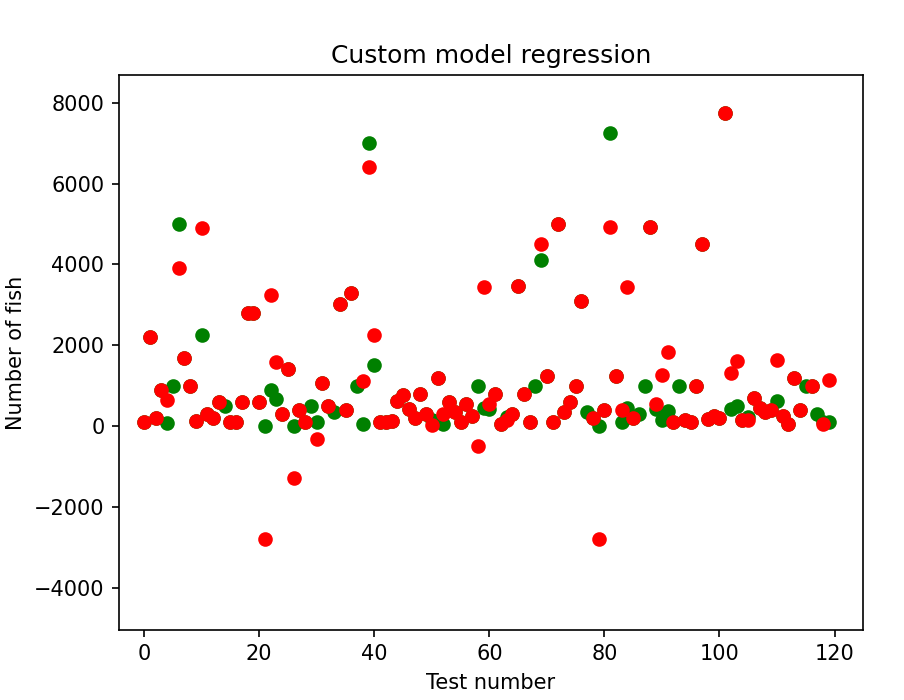
\includegraphics[width=0.8\linewidth]{Custom model regression.png}
\caption{Przewidywane wartości dla modelu customowego}
\label{fig:wykres_customowej_regresji}
\end{center}
\end{figure}

Oprócz \ref{eq:wzor_customowej_regresji} zostały także użyte modele liniowy i SVR

Dzięki funkcjom mean\_squared\_error oraz mean\_absolute\_percentage\_error z modułu sklearn zostały wyliczone błedy kwadratowe i procentowe poszczególnych medeli regresji, aby sprawdzić ich skuteczność.

\section{Wnioski}
Przedstawiony program pozwala na dobranie optymalnego modelu regresji do przewidzenia liczby ryb użytych do zarybienia zbiornika wodnego. Po kilku próbach, dla różnych wielkości danych widać skuteczność modelu SVR niezależnie od liości wykorzystanych wierszy, wierszy skuteczność modelu liniowego dla mniejszej liczby wierszy oraz potrzebę większej liczby wierszy dla własnego modelu regresji. 

Zależnie od liczby wierszy wziętych do stworzenia modeli, model liniowy osiąga zazwyczaj błąd procentowy(mean absolute percentage error) rzędu kilku procent dla danych nie przekraczających 300 wierszy i kilka milionów procent dla danych przekraczających 300 wierszy. 

Model SVR niezależnie od wielkości danych, osiąga błąd procentowy(mean absolute percentage error) od 0,5 do 6 procent. Dla większej liczby danych, model lepiej się uczy i osiąga coraz mniejszy błąd.

Model własny potrzebuje danych posiadających kilkaset wierszy żeby zadziałał, ponieważ liczba kolumn musi być mniejsza niż liczba wierszy, dlatego przy danych posiadających 600 wierszy, model customowy osiąga błąd procentowy(mean absolute percentage error) rzędu kilkudziesięciu procent.

\appendix
\section{Dodatek}
Kody źródłowe(utrzymane w konwencji języka Python wraz z instrukcjmi uruchomienia) umieszczone zostały w repozytorium github:

\noindent \url{https://github.com/Drysiek/Fish-Stock-Regression}.

\end{document}